\documentclass[addpoints]{exam}
\usepackage{amsmath,amsthm,amssymb,url}

\usepackage{algorithm}
\usepackage{algorithmic}
\usepackage{graphicx}
\usepackage{float}
\usepackage[pdftex]{hyperref}
\usepackage{tikz}
\usetikzlibrary{positioning}
\tikzset{main node/.style={circle,fill=blue!20,draw,minimum size=1cm,inner sep=0pt},
            }
\def\checkmark{\tikz\fill[scale=0.4](0,.35) -- (.25,0) -- (1,.7) -- (.25,.15) -- cycle;} 
\def\cov{\mathrm{Cov}}
\newcommand{\Exval}[1]{\left< #1\right>}
\newcommand{\ExvalDef}[1]{\sum_{i=0}^{\infty} #1P\left( #1\right)}
\newcommand{\Var}[1]{\sigma^{2}\left( #1\right)}
\newcommand{\VarDef}[1]{\left< #1^{2}\right> - \left< #1\right>^{2}}
\newcommand{\BigO}[1]{\mathcal{O}\left( #1\right)}
\newcommand{\BigT}[1]{\Theta\left( #1\right)}
\newcommand{\BigOmega}[1]{\Omega\left( #1\right)}
\newcommand{\T}[1]{T\left( #1\right)}
\renewcommand{\P}[1]{\left( #1\right)}
\newcommand{\floor}[1]{\lfloor #1\rfloor}
\newcommand{\ceil}[1]{\left\lceil #1\right\rceil}
\newcommand{\Lim}[1]{\raisebox{0.5ex}{\scalebox{0.8}{$\displaystyle \lim_{#1}\;$}}}
\newcommand{\abs}[1]{\left| #1\right|}


\newtheorem{lemma}{Lemma}[section]
\newcommand{\var}{\text{Var}}
\title{CS 6150: Homework 3}
\date{Due Date: October 30, 2015}
\author{Christopher Mertin\\{\scriptsize (P.S. I did this while drunk)}}
\begin{document}
\maketitle
\begin{center}
\fbox{\fbox{\parbox{5.5in}{\centering
This assignment has \numquestions\ questions, for a total of \numpoints\
points.
Unless otherwise specified, complete and reasoned arguments will be expected for all answers. }}}
\end{center}

\qformat{Question \thequestion: \thequestiontitle\dotfill \textbf{[\totalpoints]}}
\pointname{}
\bonuspointname{}
\pointformat{[\bfseries\thepoints]}

\printanswers

\begin{center}
  \gradetable
\end{center}
\newpage



\begin{questions}

\titledquestion{Minimum-cost Tree}

In this problem, the input consists of a complete graph $G=(V,E)$ with distances between all pairs of vertices, and a set $V'\subseteq V$.
Suppose the distances in the input is a metric, and the weight of an edge connecting two vertices in $G$ is defined as the distance between these two vertices.
\begin{parts}



  \part[20] Design  a ratio-2 approximation algorithm to find a minimum-cost tree that includes $V'$. The cost of a tree is the sum of all weights
  of its edges. This tree may or may not include vertices in $V-V'$. Show the approximation ratio of your algorithm is 2. (Hint: Recall the approximation algorithm for the TSP.)


\begin{algorithm} % enter the algorithm environment
\begin{algorithmic}% enter the algorithmic environment
\STATE label $v$ as discovered
\FORALL{edges $w$ {\bf in} $G$.adjacentEdges($v$)} \IF{vertex $w$ is not labeled as discovered} \STATE{recursively call DFS($G$,$w$)} \ENDIF \ENDFOR
\end{algorithmic}
\caption{DFS($G$,$v$):}
\label{alg:DFS}
\end{algorithm}

\begin{solution}
Before solving this, the Depth-First-Search (DFS) Algorithm is required which can be seen in Algorithm~\ref{alg:DFS}.

We want to find a minimum-cost spanning tree $V^{\prime}$ such that $\text{cost}(OPT)\leq \text{cost}(V^{\prime})\leq 2\text{cost}(OPT)$

This can be done by creating an empty list $\Omega$ which will store the approximation of the minimum-cost tree. We can do this by running the DFS at the start of the root node and adding it to $\Omega$ whenever a vertex is pre-visited or returned to after the recursive call. This will essentially {\em double} the nodes in the tree, however this is what is desired. For example, if we wanted to describe a cycle with the nodes in $\Omega$, then DFS would use the cost twice. This would force the {\em max cost} to be $2\text{cost}(OPT)$, thus providing the upper bound.

This can be made closer to the lower bound of $OPT$ by removing all the vertices that are in $\Omega$ but not in $V^{\prime}$, which is by $V-V^{\prime}$. As the weights must be positive, there is no way for this to add to the overall cost and should only decrease it. Following this, all but the first instances of each node in $\Omega$, which will be a cycle where each node in $V^{\prime}$ will only be traversed once. Finally, as it's a cycle, any edge at random will produce a spanning tree that approximates the minimum-cost. Since we started at $2\text{cost}(OPT)$ and removed edges, we can say that we are far below than this now, bounding the problem by $V^{\prime}$ being $\text{cost}(OPT)\leq \text{cost}(V^{\prime})\leq 2\text{cost}(OPT)$.

\end{solution}


\end{parts}




\titledquestion{Max-SAT Problem}

Suppose you are given a set of clauses, and each clause is the the disjunction of several literals. Your goal is to find an assignment that satisfies as many of these clauses as possible.

\begin{parts}

  \part[8] Here is a simple algorithm:

\begin{algorithm} % enter the algorithm environment
\begin{algorithmic} % enter the algorithmic environment
\FOR { each variable}
\STATE {set its value to either 0 or 1 by flipping a coin}
\ENDFOR
\end{algorithmic}
\end{algorithm}
Suppose the input has $m$ clauses, of which the $j$th has $k_j$ literals, show that the expected number of clauses satisfied by the above algorithm is no less than $\frac{m}{2}$. In other words, this is a $2$-approximation in expectation.

\begin{solution}
To find the bound, we can look at the probability of this happening for the case of only one literal being true. This can be done as the following.

Without loss of generality, we can assume that the literals are ordered in the way that they appear. For example, the very first literal to appear will be labeled as $x_{1}$, the next as $x_{2}$, and so on until we get to the $n^{th}$ literal. This notation will help in understanding the proof.

Assume that the first literal $(x_{1})$ is such that the first clause is true. As this is independent, and the bits are set randomly, the probability of the first clause being true is $\frac{1}{2}$. 

This can be extended down through each of the $m$ clauses, as each are independent. This turns into being a sum of $\sum_{i=1}^{m}\frac{1}{2}=\frac{m}{2}$. As this is the {\em lower bound} for one literal being true, any more literals would make it increase and the above algorithm would be no less than $\frac{m}{2}$. 
\end{solution}
\part[12] Improve the above algorithm to make it deterministic.

\begin{solution}

This algorithm can be changed to be deterministic to increase the maximum number of clauses. 

To make this deterministic, we can set all of the bits to $0$. With using the labeling convention that was stated in part $(a)$, we can iterate through each bit and check the number of clauses that it makes true. In other words, take $x_{1}$ and since it is zero, we check to see how many clauses it makes true, and then we flip it on and check how many are true. We choose to if it is on or off based on the {\em maximum} number of clauses that are true. For example, if when $x_{1}$ was off only 3 clauses were true and when $x_{1}$ was on 17 were true, we choose $x_{1}$ to be on. We iterate through all of the literals and treat them all like this. This will result in a deterministic algorithm that is done in $\BigO{n}$.
\end{solution}

\end{parts}





\titledquestion{Containers and Truck}
 Suppose a ship arrives, with $n$ containers of weight $w_1,w_2,\cdots,w_n$. Standing on the dock is a set of trucks, each of which can hold $K$
 unites of weight. (You can assume that $K$ and each $w_i$ is an integer.) You can stack multiple containers in each truck, subject to the weight
 restriction of $K$; the goal is to minimize the number of trucks that are needed in order to carry all the containers.
 
 A greedy algorithm you might use for this is the following. Start with an empty truck, and begin piling containers $1, 2, 3, \ldots $ into it until you get to a container that would overflow the weight limit. Now declare this truck "loaded" and send it off; then continue the progress with a fresh truck. This algorithm, by considering trucks one at a time, may not achieve the most efficient way to pack the full set of containers into an available collection of trucks.
 

\begin{parts}
  \part[5] Give an example of a set of weights, and a value of $K$, where this algorithm does not use the minimum possible number of trucks.

\begin{solution} $K$ is defined as the max load of the truck and $W$ is the set of items that holds their corresponding weights. 
\begin{align*}
K &= 1000\ kg\\
W &= \{ 999\ kg, 2\ kg,999\ kg,2\ kg,999\ kg,2\ kg,999\ kg,2\ kg  \}
\end{align*}

The truck would have to make a new run with each item as to not overload the truck, resulting in 8 truck runs which is not the optimal.
\end{solution}
  
  \part[15] Show, however, that the number of trucks used by this algorithm is within a factor of  $2$ of the minimum possible number, for any set of weights and any value $K$.

\begin{solution}
The optimal run would be to take as many objects as possible in each run, similar to the knapsack problem. The absolute worst case scenario is the above case that was given as a solution to $(a)$ in which they are evenly distributed such that each load item will have to be a new delivery. This makes sense because if there were multiple small items inbetween each heavy item, one truck could take more than one of them, thus lowering the bound. Therefore, if this case is less than 2 times the optimal, then so will every other case. We can prove that the $\text{cost}(worst) \leq 2\text{cost}(OPT)$ with a proof by contradiction. Assume the worst case is such that $\text{cost}(worst) > 2\text{cost}(OPT)$.

In the case of $OPT$, if the sum of all the small boxes were within the max load of the truck, it would be able to take all of them in a single load. If the total number of boxes is $n$, then the optimal solution would only make $\BigOmega{\frac{n}{2}+1}$ truck loads as it has to take one at a time for the larger boxes, where $2\text{cost}(OPT) = \BigOmega{n+2}$ then. This is trivially proven because it is impossible to take more than $n$ trips to deliver $n$ items, as long as all the items are individually within the weight limit of the truck. As it cannot be proven to be greater than $n+2$, the contradiction is false and the statement $\text{cost}(worst) \leq 2\text{cost}(OPT)$  must be true.

\end{solution}
  
  
\end{parts}




\titledquestion{Grid Graph}

   Suppose you are given an $n\times n$ grid graph $G$ as in the following figure.

\begin{figure}[H]
  \centering
  % Requires \usepackage{graphicx}
  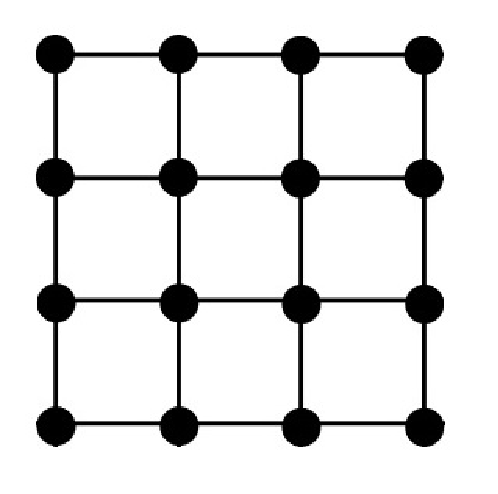
\includegraphics[width=0.3\textwidth]{fig1.pdf}\\
  \caption{A grid graph.}
\label{fig:nxn}
\end{figure}

Associated with each node $v$ is a weight $w(v)$, which is a nonnegative integer. You may assume that the weights of all nodes are distinct.
Your goal is to choose an independent set $S$ of nodes of the grids, so that the sum of the weights of the nodes on $S$ is as large as possible.
(The sum of the weights of the nodes in $S$ will be called its total weight.)


Consider the following greedy algorithm for this problem.
\begin{algorithm*} % enter the algorithm environment
\caption{The "heaviest-first" greedy algorithm:} % give the algorithm a caption
\begin{algorithmic} % enter the algorithmic environment
\STATE Start with $S$ equal to the empty set
\WHILE {some node remains in $G$}
\STATE Pick a node $v_i$ of maximum weight
\STATE Add $v_i$ to $S$
\STATE Delete $v_i$ and its neighbors from $G$
\ENDWHILE
\RETURN $S$
\end{algorithmic}
\label{alg:Heavy}
\end{algorithm*}



  \begin{parts}
    \part[7] Let $S$ be the independent set returned by the "heaviest-first" greedy
    algorithm, and let $T$ be any other independent set in $G$. Show that, for each node $v\in T$,
    either $v\in S$, or there is a node $v'\in S$ so that $w(v)\leq w(v')$ and $(v,v')$ is an edge of $G$.

\begin{solution}
This can be proven via {\em Proof by Contradiction}

Suppose $v\in T$ and $v\notin S$, and that $v$ does not have a neighbor $v^{\prime}\in S$ such that $w(v)\leq w(v^{\prime})$. Because of this second relation, we know that one of $v$'s neighbors has to be in $S$, so for the proof assume $v^{\prime}$ is $v$'s neighbor. Then, when $v^{\prime}$ is added to $S$, $v$ must still be on the graph because the largest weighted neighbor of $v$ was $v^{\prime}$, so it goes to also show that $v\notin S$.

However, according to Algorithm~\ref{alg:Heavy}, $v^{\prime}$ cannot be added to $S$ at this time as $w(v) > w(v^{\prime})$. This leads to a contradiction, so for each node $v\in T$, either $v\in S$ or there is another node $v\in S$ such that $w(v)\leq w(v^{\prime})$ where $(v,v^{\prime})$ is an edge in $G$.

\end{solution}

    \part[13] Show that the "heaviest-first" greedy algorithm returns an independent set of total
    weight at least $\frac{1}{4}$ times the maximum total weight weight of any independent set in the grid graph $G$.

\begin{solution}
From Figure~\ref{fig:nxn}, it can easily be seen that any node in $G$ has at most $4$ neighbors. Therefore, for any independent set of nodes $T$, a maximum of $4$ nodes in $T-S$ can share one node from $S-T$ as a common neighbor. This comes from part $(a)$, as an element in $T$ cannot exist in $S$ and vice versa. Therefore, we can say

\begin{align*}
\sum_{v\in T}w(v) &= \sum_{v\in T\cap S}w(v) + \sum_{v\in T-S}\\
				&\leq \sum_{v^{\prime} S\cap T}w(v^{\prime}) + 4\sum_{v^{\prime}\in S-T}w(v^{\prime}) \leq 4\sum_{v^{\prime}\in S}w(v^{\prime})
\end{align*}



Thus, the above algorithm gives a value that is $\frac{1}{4}$ times the size of the total weight of the total graph in the {\em minimum} case.
\end{solution}

  \end{parts}

\titledquestion{Graph Coloring}[20]

Solve Question 8, parts (a), (b) \textbf{ONLY} from
\url{http://web.engr.illinois.edu/~jeffe/teaching/algorithms/notes/31-approx.pdf}. Each
part is worth 10 points. 

\begin{solution}
Part a

{\bf Bipartitle Graph:} A graph whose vertices can be divided into two disjoint sets.

The given graph is said to be bipartite. Assume that it can't be colored with only two colors. As it is bipartite, it can be separted into two disjoint sets and all but the last node can be colored trivially with only two colors since the sets are disjoint by simply following the algorithm. The potential problem comes when deciding on the color of the last node.

When looking at the last node, in the first if statement it will look at the colors of the nodes that neighbor $u$, and since the graph is disjoint, all of the nodes/neighbors that connect to $u$ are on the physical side of $v$, so it will get the opposite color of those. The same goes when trying to color $v$, as the set is disjoint, all connecting neighbors will be on the physical side of $u$ and thus $v$ will be colored the opposite color of them. These two results {\em must} hold true since the graph is bipartite. Therefore, the third if statement won't be implemented and the graph can be colored in only two colors.

There's also the fact that since the graph is bipartite, if it couldn't be colored into two disjoint sets it would violate the definition of it being bipartitle, thus also proving it true.

\end{solution}

\begin{solution}
Part b: $\Delta G$ denotes the maximum degree of any vertex in $G$.

This can be proved via induction

The given algorithm colors the edges/nodes based on the surrounding ones. So, for the base case, if the maximum degree was 1 ($\Delta G = 1$), theree would only need to be one color as it's restricted to two nodes.

Assume that this holds true up to $\Delta G = n$, such that only $n$ colors are needed to color the graph. For $\Delta G  = n+1$, this would be done by taking the same graph in the $\Delta G = n$ case and attaching an edge to the vertex with degree $n$ to another vertex. To label this, as from the algorithm, by induction the node $\Delta G$ contains all the colors in the graph, so no colors in the surrounding set will work. Therefore, a new color has to be made, thus making it $n+1$ approximate.


\end{solution}


\textbf{BONUS:} for 10 extra points, solve Question 8(c). Note that you will
solve this by constructing an example graph of size $n$ and showing that you
need $\omega(1)$ colors. 

\begin{solution}
As stated as the solution in part $(b)$, the number of colors used is equal to the node with the highest degree. However, the optimal solution comes from the {\em Four-Color Theorem} which states that any ``map in a plane can be colored by using four-colors in such a way that regions sharing a common boundary (other than a single point) do not share the same color'' with the use of only four colors \cite{wolfram}. As it is based on the size of the max degree, it is not a constant factor as it is in the {\em Four-Color Theorem}.
\end{solution}


\end{questions}


\begin{thebibliography}{99}
\bibitem{wolfram} Weisstein, Eric W. ``Four-Color Theorem." From MathWorld--A Wolfram Web Resource. \url{http://mathworld.wolfram.com/Four-ColorTheorem.html}
\end{thebibliography}

\end{document}
